% Rapport de remise -- compiler depuis la racine : tectonic docs/rapport-final.tex --outdir docs
\documentclass[11pt,a4paper]{article}
\usepackage[french]{babel}
\usepackage{fontspec}
\setmainfont{Georgia}
\setsansfont{Avenir Next}
\usepackage{geometry}
\geometry{top=19mm,bottom=20mm,left=21mm,right=21mm}
\usepackage{microtype}
\usepackage{graphicx}
\usepackage{booktabs,tabularx,array}
\usepackage{enumitem}
\usepackage{fancyhdr}
\usepackage{hyperref}
\usepackage{xcolor}
\usepackage{titlesec}
\usepackage{needspace}
\definecolor{bleu}{HTML}{17345C}
\definecolor{turquoise}{HTML}{087F8C}
\definecolor{gris}{HTML}{526172}
\definecolor{pale}{HTML}{EDF4F7}
\hypersetup{colorlinks=true,linkcolor=bleu,urlcolor=turquoise,pdftitle={Vélib' Métropole -- analyse de la disponibilité à 30 minutes},pdfauthor={Akram Ghazlouny, Youssef Ejjiyar, El Mehdi Ben Yahya, Ahmed Hussein}}
\titleformat{\section}{\Large\sffamily\bfseries\color{bleu}}{\thesection}{0.6em}{}
\titleformat{\subsection}{\large\sffamily\bfseries\color{bleu}}{\thesubsection}{0.6em}{}
\pagestyle{fancy}
\fancyhf{}
\fancyhead[L]{\footnotesize\sffamily Vélib' Métropole · Kit Data Science}
\fancyhead[R]{\footnotesize\sffamily 7 novembre 2026}
\fancyfoot[C]{\footnotesize\thepage}
\renewcommand{\headrulewidth}{0.4pt}
\setlength{\headheight}{14pt}
\setlength{\parskip}{0.45em}
\setlength{\parindent}{0pt}
\setlength{\emergencystretch}{2em}
\setlist[itemize]{leftmargin=1.5em,itemsep=0.15em,topsep=0.15em}
\newcommand{\source}[1]{\textsuperscript{\color{turquoise}[#1]}}
\newcommand{\callout}[1]{\noindent\colorbox{pale}{\parbox{\dimexpr\linewidth-2\fboxsep\relax}{\vspace{0.4em}#1\vspace{0.4em}}}}

\begin{document}
\thispagestyle{empty}
\vspace*{19mm}
{\sffamily\large\color{turquoise} DATA-IA-EXE710 · Télécom Paris · Projet de groupe\par}
\vspace{6mm}
{\sffamily\bfseries\fontsize{25}{31}\selectfont\color{bleu} Vélib' Métropole : peut-on prévoir une station vide dans 30 minutes ?\par}
\vspace{7mm}
{\Large Une évaluation temporelle fondée sur les relevés réels du 25 au 30 octobre 2026\par}
\vspace{12mm}
\callout{\textbf{Réponse courte.} La cible « station en service et sans vélo exactement à +30 minutes » est mesurable lorsque les deux relevés existent. Sur le test chronologique, la forêt aléatoire atteint un F1 de \textbf{0,564}, contre \textbf{0,562} pour la simple persistance de l'état actuel. Ce gain de 0,002 ne permet pas d'affirmer que le modèle améliore la prévision. Parmi les stations encore pourvues de vélos, le rappel n'est que de \textbf{10,0\,\%} pour la forêt. Il s'agit d'une preuve de concept, pas d'un système d'alerte fiable.}
\vfill
{\sffamily\bfseries Auteurs\par}
Akram GHAZLOUNY · Youssef EJJIYAR · El Mehdi BEN YAHYA · Ahmed HUSSEIN\\
\vspace{4mm}
\textbf{Version de remise :} \href{https://github.com/G-Akram01/velib-kit-data-science/tree/finalisation-remise-2026-11-08}{branche \texttt{finalisation-remise-2026-11-08}}\\
\textbf{Notebook :} \href{https://colab.research.google.com/github/G-Akram01/velib-kit-data-science/blob/finalisation-remise-2026-11-08/notebooks/Analyse_velib_V_07_11.ipynb}{ouvrir la version vérifiée dans Google Colab}\\
\textbf{Date de remise annoncée dans le dépôt :} 8 novembre 2026, 18 h (heure de Paris).
\newpage

\section{Question, périmètre et critères de réponse}

La question du projet est : \emph{une station Vélib' en service à l'instant $t$ sera-t-elle vide exactement 30 minutes plus tard ?} Nous définissons « vide » par zéro vélo disponible et \texttt{is\_renting=1}. Une station où l'emprunt est interdit n'est pas assimilée à une station vide : la situation est différente pour l'usager et pour l'analyse. Les données sont des instantanés de stations, pas des trajets individuels.

Le notebook principal retient uniquement les couples station--instant pour lesquels un relevé existe à $t$ et à $t+30$ minutes et pour lesquels l'emprunt est autorisé aux deux instants. La cible vaut 1 lorsque le nombre de vélos à $t+30$ est nul. Cette sélection garantit une étiquette observée, mais elle restreint la réponse : une station ouverte à $t$ puis fermée à $t+30$ est exclue \emph{a posteriori}. La prédiction opérationnelle de toute indisponibilité, y compris une fermeture future, n'est donc pas étudiée ici.

\callout{\textbf{Critère de réussite scientifique.} Dépasser clairement une règle de référence sur un test chronologique distinct, surtout pour les stations qui ont encore des vélos au moment de la prédiction. Un score élevé sur toutes les stations peut simplement reconnaître celles qui sont déjà vides.}

\section{Données, qualité et gouvernance}

Le collecteur conserve les flux publics GBFS \texttt{station\_status.json} et \texttt{station\_information.json} de Vélib' Métropole sous forme de JSON compressé, avec l'heure UTC de collecte et l'URL source. Le référentiel utilisé pour la jointure est figé au 25 octobre 2026. Le catalogue Paris Data décrit les données de disponibilité comme dynamiques et indique Smovengo/Syndicat Autolib' Vélib' Métropole comme producteur ; sa fiche affiche la licence ODbL pour \emph{ce jeu de données catalogué}.\source{1} Les conditions applicables directement au flux GBFS doivent être vérifiées avant une redistribution autonome. L'attribution de la source et la date de consultation sont conservées dans la \href{https://github.com/G-Akram01/velib-kit-data-science/blob/finalisation-remise-2026-11-08/docs/gouvernance-donnees.md}{note de gouvernance et le dictionnaire des variables}.

\begin{center}
\begin{tabularx}{\linewidth}{@{}Xr@{}}
\toprule
\textbf{Contrôle sur la période retenue} & \textbf{Valeur}\tabularnewline
\midrule
Créneaux de cinq minutes observés / attendus & 1\,736 / 1\,740 (99,8\,\%)\\
Interruptions entre relevés & 4 trous de 10 min\\
Lignes station $\times$ relevé avant exclusions & 2\,637\,708\\
Stations avec signalement de plus de 24 h exclues & 17\\
Stations analysées après exclusion & 1\,503\\
Observations de stations en service sans vélo & 4,8\,\%\\
\bottomrule
\end{tabularx}
\end{center}

Le 25 octobre comporte 25 heures en raison du passage à l'heure d'hiver : 300 créneaux théoriques ce jour-là. Les doublons station--créneau sont résolus en conservant la collecte la plus récente ; les observations futures manquantes ne sont pas interpolées. L'audit glissant des 48 heures précédant le dernier relevé du 7 novembre trouvait seulement 9 instantanés sur 576 attendus (1,56\,\%). Ces données récentes, trop discontinues, ne sont pas mélangées aux six jours denses.

La gouvernance du projet distingue les données brutes, le référentiel, les contrôles qualité et la vue calculée dans le notebook. Aucun identifiant d'usager ni trajet individuel n'est enregistré. Les fichiers bruts restent versionnés et les règles de nettoyage sont documentées ; une conservation plus longue nécessite un stockage et une durée d'archivage explicitement définis.

\clearpage
\section{Fermetures temporaires : contexte et biais}

La Ville de Paris a annoncé 110 stations Vélib' fermées pour les manifestations du 24 octobre, avec réouverture progressive dans la nuit du 25 au 26.\source{2} Vélib' Métropole a annoncé 110 fermetures pour celles du 31 octobre, effectives dès le vendredi 30.\source{3} Il s'agit de fermetures de précaution liées aux manifestations ; les données du projet ne permettent pas de qualifier chaque fermeture de « grève » ni d'en attribuer la cause individuelle.

Dans les relevés du projet, les stations avec \texttt{is\_renting != 1} sont environ 166 le dimanche 25, environ 20 en milieu de semaine et jusqu'à 142 en fin de journée le 30. La concordance temporelle avec les annonces est forte, mais le compteur GBFS agrège aussi d'autres raisons possibles de fermeture. Les taux de stations vides du notebook portent seulement sur celles où l'emprunt est possible. Le dimanche observé et la fin du test ne représentent pas nécessairement des conditions habituelles.

\begin{figure}[ht]
\centering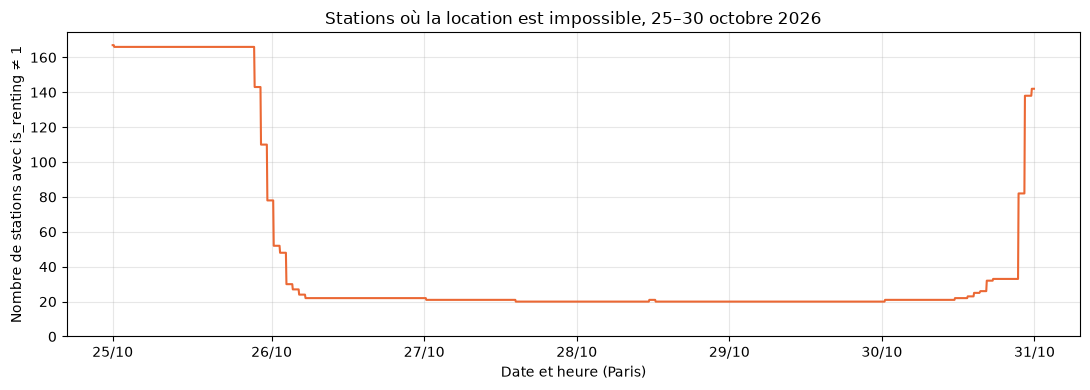
\includegraphics[width=0.88\linewidth]{figures/fermetures.png}
\caption{Stations où la location est impossible dans les instantanés conservés. La courbe ne fournit pas la cause de l'indisponibilité. Source : calculs du notebook sur les flux GBFS archivés.}
\end{figure}

\section{Méthode de prévision et évaluation}

Les variables explicatives décrivent l'état présent (vélos, bornes libres, types, taux de remplissage), les variations à 15 et 30 minutes passées, l'heure, le week-end, les coordonnées et la fréquence historique de vide de chaque station. Cette dernière est calculée sur l'entraînement seul. Les valeurs historiques absentes sont remplacées par zéro : cette simplification peut masquer une variation inconnue. Aucune variable mesurée après $t$ n'entre dans les modèles.

L'ensemble est découpé dans l'ordre du temps : entraînement jusqu'au 28 octobre à 13 h 05, validation du 28 octobre à 13 h 40 au 29 octobre à 10 h 45, test du 29 octobre à 11 h 20 au 30 octobre à 23 h 25. Un écart de 30 minutes avant chaque coupure empêche les étiquettes d'une période de déborder sur la suivante. Le test comporte 640\,191 couples station--instant ; les seuils des classifieurs sont choisis sur la validation uniquement. L'entraînement des deux modèles utilise un échantillon reproductible de 300\,000 lignes. Le comparateur « persistance » prédit qu'une station vide maintenant sera encore vide à +30 minutes.

\begin{center}
\textbf{Résultats sur toutes les stations du test}\par\smallskip
\begin{tabular}{@{}lrrrr@{}}
\toprule
Modèle & Précision & Rappel & F1 & PR-AUC\\
\midrule
Persistance & 0,560 & 0,565 & 0,562 & --\\
Régression logistique & 0,526 & 0,577 & 0,550 & 0,526\\
Forêt aléatoire & 0,550 & 0,579 & 0,564 & 0,582\\
\bottomrule
\end{tabular}
\end{center}

\Needspace{5\baselineskip}
La forêt aléatoire produit 16\,034 vrais positifs, 13\,123 faux positifs et 11\,673 faux négatifs, pour 599\,361 vrais négatifs. Elle manque donc plus de 11\,000 événements « vide » dans ce seul test, malgré un F1 global voisin de la persistance. La PR-AUC mesure le classement des risques ; elle ne transforme pas à elle seule ces prédictions en alertes utiles à un seuil choisi.

\begin{center}
\textbf{Sous-ensemble initialement non vide : passage à vide à +30 min}\par\smallskip
\begin{tabular}{@{}lrrrr@{}}
\toprule
Modèle & Précision & Rappel & F1 & PR-AUC\\
\midrule
Persistance & 0,000 & 0,000 & 0,000 & --\\
Régression logistique & 0,253 & 0,084 & 0,126 & 0,185\\
Forêt aléatoire & 0,342 & 0,100 & 0,155 & 0,219\\
\bottomrule
\end{tabular}
\end{center}

Cette seconde table répond mieux au besoin d'anticipation : la forêt prédit correctement environ un tiers de ses alertes, mais ne repère qu'environ un passage à vide sur dix. La régression logistique en repère encore moins, avec une précision plus faible. Les résultats sont issus d'une seule coupure temporelle et de six journées d'automne ; ils ne mesurent pas la stabilité entre semaines ou en période sans manifestations.

\begin{figure}[ht]
\centering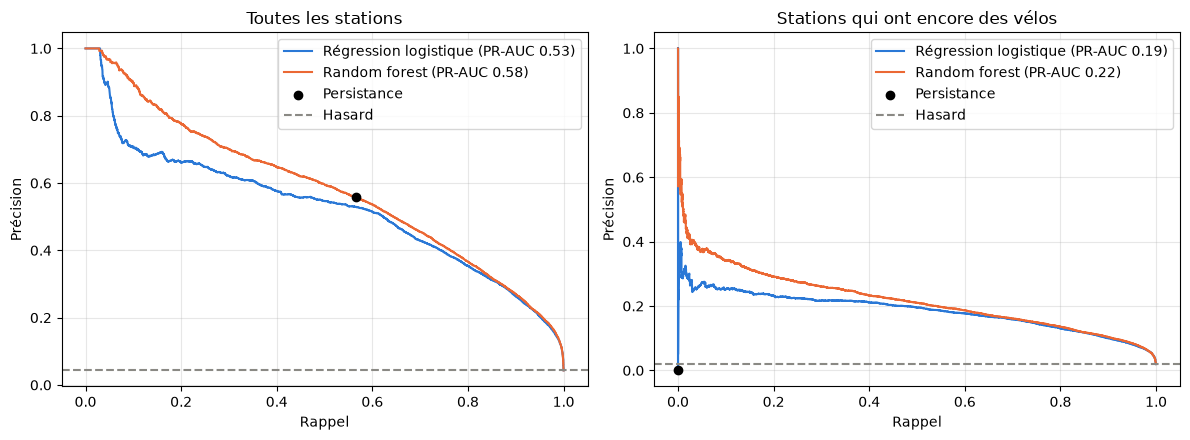
\includegraphics[width=0.92\linewidth]{figures/precision-rappel.png}
\caption{Courbes précision--rappel du notebook principal : toutes les stations à gauche, stations initialement non vides à droite. Les seuils présentés dans les tables ont été fixés sur la validation.}
\end{figure}

\clearpage
\section{Réponse et portée des résultats}

\callout{\textbf{Conclusion.} Oui, le projet sait \emph{construire} une cible exacte à +30 minutes et évaluer des modèles sur des relevés réels. Non, il ne démontre pas aujourd'hui une prévision fiable des stations qui vont se vider : le gain global de la forêt sur la persistance est négligeable et le rappel des nouveaux passages à vide est faible. Les stations fermées dans les 30 minutes suivantes sont hors du champ de l'évaluation.}

Une régression complémentaire du nombre de vélos obtient une erreur absolue moyenne de 1,46 vélo, contre 1,34 pour la règle « nombre de vélos inchangé ». Elle n'apporte donc pas de gain établi. Le notebook \texttt{03\_Machine\_Learning\_Modeling.ipynb} étudie une cible différente (« à un moment quelconque des 30 prochaines minutes ») ; ses scores ne sont pas comparés aux chiffres ci-dessus.

\subsection{Limites qui orientent la suite}
\begin{itemize}
\item \textbf{Période et incidents.} Six jours, un seul dimanche et deux épisodes de fermeture encadrant la période ne suffisent pas à conclure sur un usage ordinaire, une saison ou l'effet des manifestations.
\item \textbf{Sélection future.} L'exclusion des stations fermées à $t+30$ utilise l'avenir pour définir la population évaluée. Elle est licite pour une analyse conditionnelle, mais ne peut être appliquée telle quelle à une alerte en temps réel.
\item \textbf{Mesure.} Le flux photographie des disponibilités, sans identifier les trajets ni la cause des fermetures. \texttt{last\_reported} n'est pas à lui seul une mesure de fraîcheur des compteurs.
\item \textbf{Généralisation.} Une seule coupure de test, un seul tirage de 300\,000 exemples d'entraînement et une collecte devenue intermittente après le 31 octobre ne permettent pas d'estimer la variabilité des performances.
\end{itemize}

\subsection{Priorités après la remise}
\begin{enumerate}[leftmargin=1.6em,itemsep=0.2em]
\item Rétablir une collecte vérifiée sur plusieurs semaines, avec alerte sur les trous et stockage adapté ; documenter les incidents de service connus.
\item Évaluer séparément les états « ouverte et vide », « ouverte et non vide » et « fermée », sans filtrer sur l'état futur pour un usage opérationnel.
\item Tester plusieurs semaines et plusieurs coupures temporelles, avec une analyse des jours perturbés, de la calibration et des faux négatifs.
\item Compléter la carte interactive et les contrôles de reproduction dans une session Colab indépendante ; valider le rendu final avec les quatre membres avant l'envoi par mail.
\end{enumerate}

\section{Reproduction et livrables}

Le dépôt public contient les instantanés, les contrôles qualité, le collecteur, les tests, le notebook exécuté et la source de ce rapport. Pour reproduire les résultats, cloner le dépôt, sélectionner la branche de remise, installer les dépendances de \texttt{requirements.txt}, lancer les tests unitaires, puis exécuter le notebook principal dans l'ordre. Depuis la racine du dépôt, compiler la source LaTeX avec Tectonic et les deux figures extraites du notebook. Les commandes exactes figurent dans le README ; les règles de provenance, nettoyage et conservation dans la note de gouvernance.

\section{État de consolidation du projet}

Le suivi des douze tâches est tenu directement dans le tableau GitHub Projects « Vélib — Planning de livraison ». Les statuts ci-dessous correspondent aux cartes mises à jour le 8 novembre 2026, sur la base des preuves présentes dans la branche de remise.

\begin{center}
\begin{tabularx}{\linewidth}{@{}lX@{}}
\toprule
\textbf{Statut Kanban} & \textbf{Tâches et raison principale}\\
\midrule
Done & \#2 qualité, \#3 préparation, \#4 exploration, \#5 preuve de concept à +30 min, \#9 évaluation, \#10 documentation.\\
Review & \#1 collecte récente dégradée ; \#6 exécution Colab propre et revue collective non prouvées ; \#11 reproduction Colab complète non prouvée.\\
In Progress & \#8 moyennes mobiles et périodes du jour absentes ; \#12 carte interactive et analyse par secteurs absentes.\\
Todo & \#7 validation du groupe et transmission effective par mail.\\
\bottomrule
\end{tabularx}
\end{center}

Le résultat négatif du modèle n'empêche pas de considérer la \emph{preuve de concept} \#5 comme réalisée. Il empêche d'annoncer un service de prévision opérationnel. La remise \#7 ne doit être validée qu'après l'envoi confirmé par le groupe.

\section*{Sources}
\begin{enumerate}[leftmargin=1.8em,label={[\arabic*]},itemsep=0.25em]
\item Paris Data, \href{https://opendata.paris.fr/explore/dataset/velib-disponibilite-en-temps-reel/information/}{« Vélib -- Vélos et bornes -- Disponibilité temps réel »}, consulté le 7 novembre 2026.
\item Ville de Paris, \href{https://www.paris.fr/?photo=26-12}{fil d'information du 23 octobre 2026 : fermetures de stations Vélib' pour les manifestations du 24 octobre}, consulté le 7 novembre 2026.
\item Vélib' Métropole, \href{https://blog.velib-metropole.fr/fermeture-temporaire-de-stations-velib-a-loccasion-des-manifestations-2/}{« Fermeture temporaire de stations Vélib' à l'occasion des manifestations »}, annonce relative au 31 octobre 2026, consultée le 7 novembre 2026.
\item Dépôt du groupe, \href{https://github.com/G-Akram01/velib-kit-data-science/tree/finalisation-remise-2026-11-08}{\texttt{G-Akram01/velib-kit-data-science}, branche de remise} ; notebook et données archivées consultés le 7 novembre 2026.
\end{enumerate}

\end{document}
